 \chapter{Metrics for Political and Emotional Engagement}

 In the following sections, we discuss the tools and methods that we use to analyze our independent variables.
 
\section{Emotional Coding}
For the emotional coding of news articles, we use dictionaries from the Harvard General Inquirer, a lexicon that is popular for computerized content analysis \cite{ stone1963computer}. The Inquirer is a public-use alternative to the LIWC system, which in Berger and Milkman’s study of online virality showed results that were significantly positively correlated with the output of manual coding \cite{berger2012makes}. In particular, we use the \emph{Positiv} and \emph{Negativ} collections, a set of 1,915 well-established words signifying positive outlook (not including words for \emph{yes}) and 2,291 words signifying negative outlook (not including words for \emph{no}), respectively. Repeating the same metrics from \emph{What Makes Online Content Viral?}, we quantify for each document:

$$ emotionality = \frac{count(positiv \mid negativ)}{count(words)}$$
$$ positivity = \frac{count(positiv)}{count(words)} - \frac{count(negativ)}{count(words)}$$

as independent variables in our analysis.

 \section{Followership as a Proxy for Political Engagement}

In the following sections, we use Twitter followership as a proxy for measuring degrees of political engagement. 

Previous research in network analysis and attempts to predict latent political affiliations of users in the social network has shown that users on Twitter tend to show network homophily within political groups, and that ``like follows like'' \cite{colleoni2014echo}. In addition, followership of only Democratic or only Republican official accounts can be used as a reasonable estimator of party loyalty. Those accounts that follow only the officials of one party tend to demonstrate more closeness with other users in their political party than those who do not.
            
Due to the highly individual nature of this election, where candidate loyalty does not necessarily imply goodwill towards the party, we look specifically at what candidates users follow instead of party loyalty at large. 

For general \emph{levels} of political engagement, we look at the number of political candidates a Twitter user follows as a proxy for how likely they are to share political news. 

In addition, for single-candidate Tweeters, we divide users by the candidate they follow. At the time of data collection completion (May 1, 2016), the top two candidates by delegate count in each party were Hillary Clinton (D), Bernie Sanders (D) and Donald Trump (R) and Ted Cruz (R), so we split users into these four groups. 

%We call each group \emph{X}-followers where \emph{X} is the candidate name, although these do not include every person on Twitter who follows \emph{X}.  

\subsection{A Look at Candidate Followership}

Our dataset contains 6,406 unique single-candidate Twitter users. Trump-only followers lead with about 31\%, followed closely by Clinton-only (29\%), then Sanders (25\%) and Cruz (14\%).


\begin{figure}[H]  
\centering 
  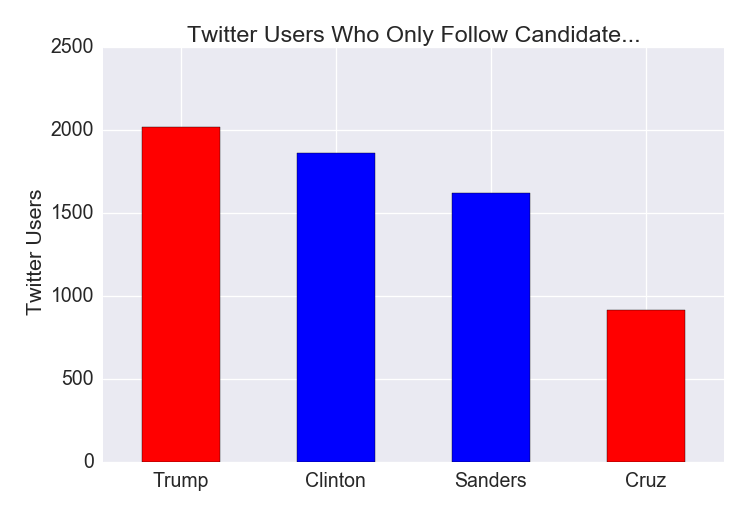
\includegraphics[width=1.0\textwidth]{users-by-candid}  
  \caption{Number of Tweets by Each Segment
    \label{fig:users-by-candid}}
\end{figure} 

 

Trump's free media advantage becomes clear when looking at the \emph{volume} of tweets each group of users tweet: 37\% of tweets sharing articles come from Trump-only followers versus 27\% for Clinton-only, 20\% for Sanders-only, and 14.6\% for Cruz.

\begin{figure}[H]  
\centering 
  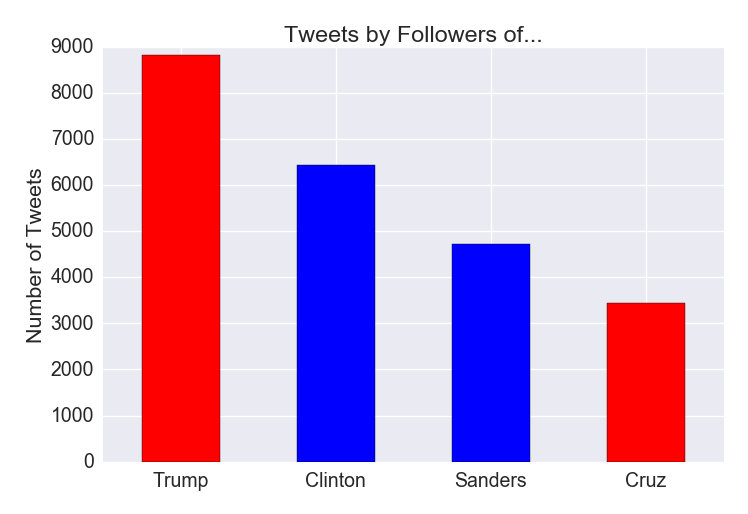
\includegraphics[width=1.0\textwidth]{tweets-by-candid}  
  \caption{Most frequently mentioned candidate in stories
    \label{fig:tweets-by-candid}}
\end{figure} 

 


Although candidate-followership is only a proxy for the latent variable of candidate loyalty, we are observe the nature of the content being shared by each group. Again, across all four segments, Republican candidate Trump leads the top number of mentions in stories shared.

%% Most popular mentioned candidate by ea. camp
\begin{figure}[H] 
\centering 
 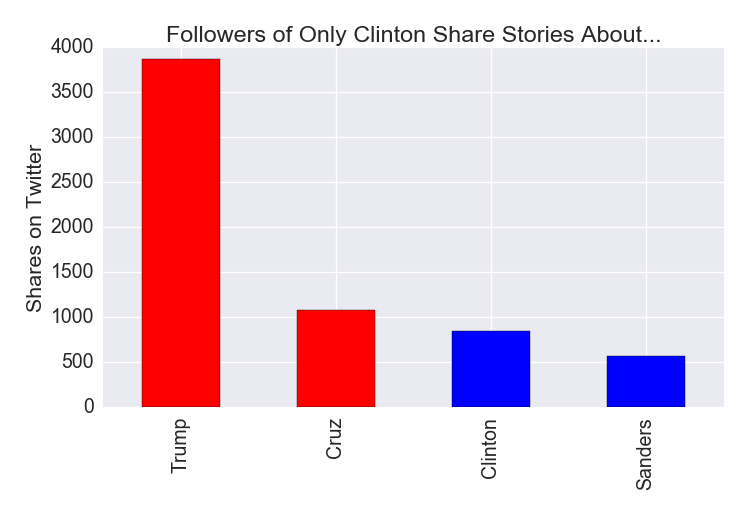
\includegraphics[width=0.49\textwidth]{clinton-camp-shares}
 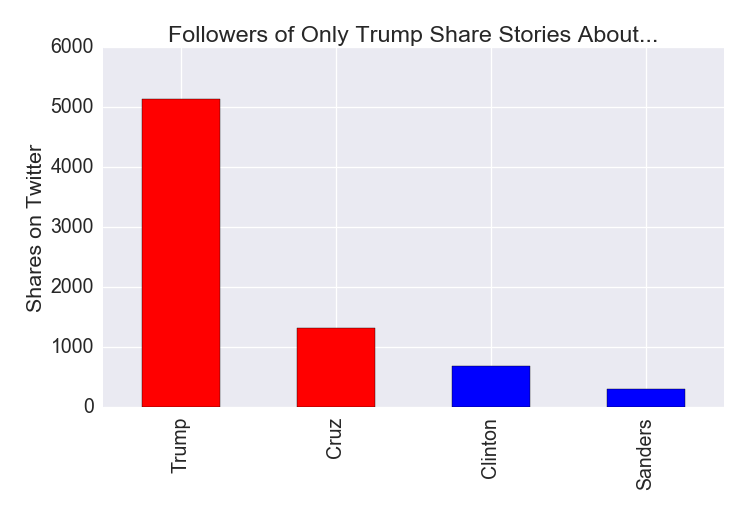
\includegraphics[width=0.49\textwidth]{trump-camp-shares}  
 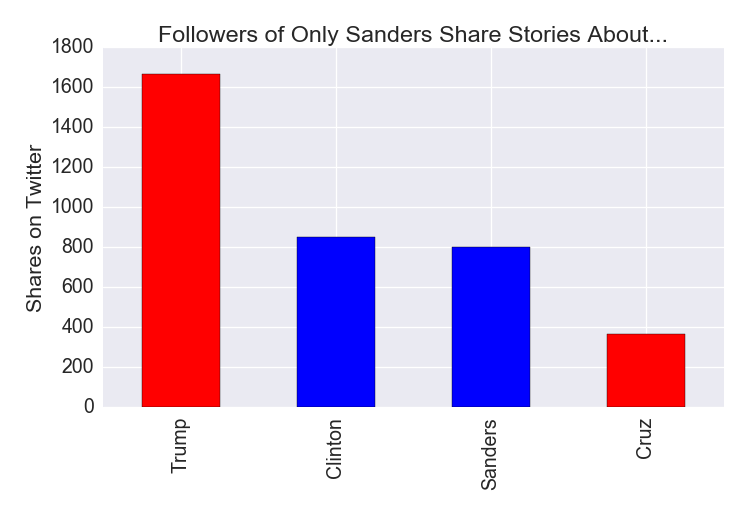
\includegraphics[width=0.49\textwidth]{sanders-camp-shares}  
 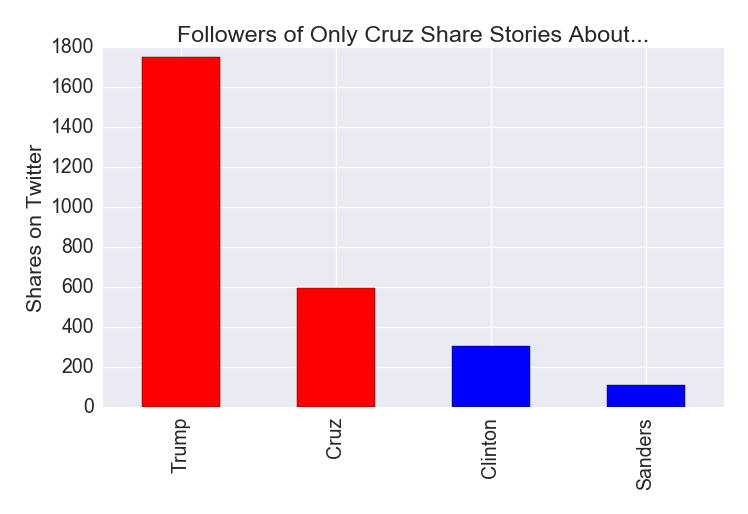
\includegraphics[width=0.49\textwidth]{cruz-camp-shares}  
  %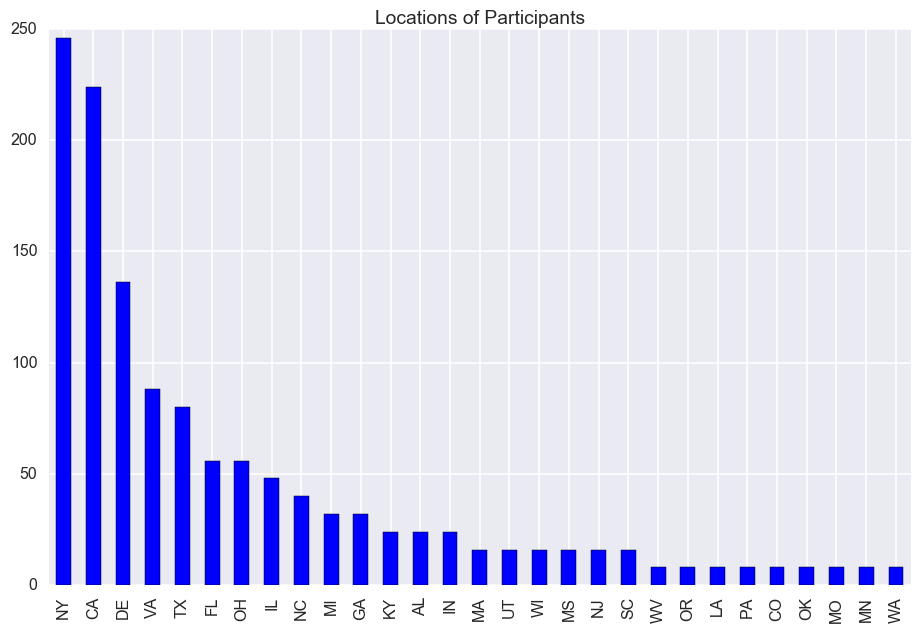
\includegraphics[width=0.32\textwidth]{location_study2} 
  \caption{Tweet and User Counts by Followership
    \label{fig:users-tweets-by-candid}}
\end{figure}
 
\subsection{A Look at Levels of Political Engagement}

% Descriptives of candididate 0/1/3+:
% * Bar chart of \% by \# Following
% * Number of tweets by each camp
% * Most popular orgs by each camp
% * Most popular story by each camp



% * Most mentioned candid in each camp


\begin{figure}[H]  
\centering 
  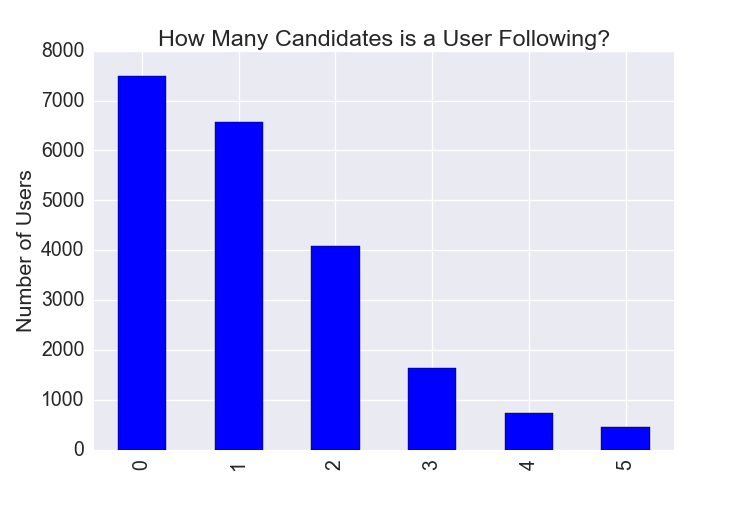
\includegraphics[width=1.0\textwidth]{candid-ct}  
  \caption{Number of candidates followed
    \label{fig:candid-ct}}
\end{figure}

36\% of Twitter users in our dataset follow none of the four political candidates, followed by 31\% who follow one candidate, 20\% who follow two, and 13\% who follow three or more candidates. 


\begin{figure}[H]  
\centering 
  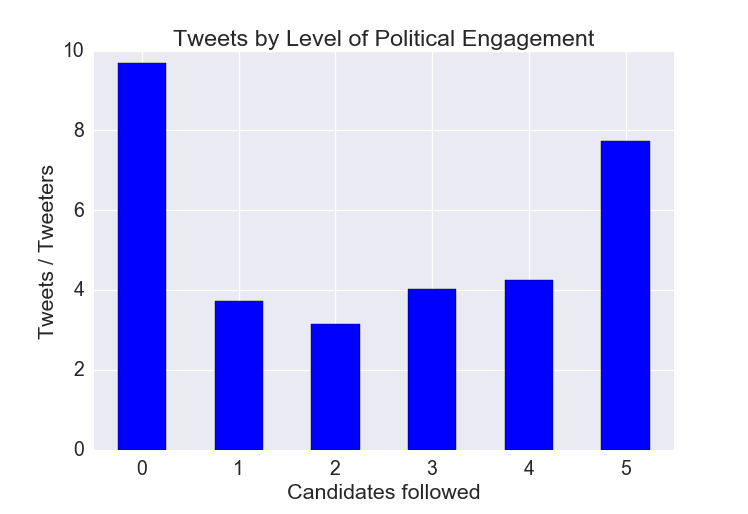
\includegraphics[width=1.0\textwidth]{tweets-by-candid-ct}  
  \caption{Ratio of Tweets to political candidates followed
    \label{fig:candid-ct}}
\end{figure}

We see a U-shaped curve between the number of candidates followed (level of observed political engagement) and the ratio of political news tweets per user.


In the following analyses, we segment levels of political engagement into three groups for the sake of comparison:

\begin{itemize}
  \item \emph{the unaffiliated} (those who follow no presidential candidates, but do tweet about political news)
  \item \emph{single-candidate} Tweeters (those who follow one and only one presidential candidate, and tweet about political news)
  \item \emph{political aficionados} (those who follow all 4 (or more) candidates, and tweet about political news)
\end{itemize}.














% * Top 10 by each camp

% %%% Trump

% \begin{table}
% \begin{tabular}{ |l c| } 
%     %s\toprule
%     \hline
%     Article &  \# tweets \\
%     \hline 
%     Donald Trump Is Shocking, Vulgar and Right                            &    221 \\
%     Trump basks in his spotlight                                          &     84 \\
%     Poll: Trump dominates GOP field                                       &     79 \\
%     The One Weird Trait That Predicts Whether You’re a Trump Supporter    &     75 \\
%     Why I'm voting for Trump                                              &     74 \\
%     Rubio: Law-abiding undocumented immigrants could stay                 &     73 \\
%     Poll: Donald Trump gained 15 points on Ted Cruz in Iowa in two weeks  &     69 \\
%     FOX NEWS POLL  Trump gains in Iowa, dominates New Hampshire           &     57 \\
%     TODD STARNES School caught trying to get students to work for Hillary &     57 \\
%     Poll: Evangelicals flocking to Trump                                  &     54 \\
%      \hline
% \end{tabular}
% \caption{\label{tab:top-10}Top 10 Shared By Trump Followers}
% \end{table}

% %%% Clinton
% \begin{table}
% \begin{tabular}{ |l c| } 
%     %s\toprule
%     \hline
%     Article &  \# tweets \\
%     \hline 
%     The One Weird Trait That Predicts Whether You’re a Trump Supporter                            &    115 \\
%     I Get Sanders’ Appeal. But He’s Not a Credible President.                                     &     74 \\
%     Ted Cruz Is No Jack Kennedy                                                                   &     68 \\
%     Why I'm voting for Trump                                                                      &     50 \\
%     Anne Frank's stepsister compares Donald Trump to Adolf Hitler                                 &     46 \\
%     Poll: Clinton has a better shot at beating Trump than Sanders                                 &     42 \\
%     Judge dismisses lawsuits over Clinton's emails                                                &     34 \\
%     Terrorists use Trump's `Muslim ban' speech in recruitment video                               &     33 \\
%     Trump’s Campaign Is Damaging His Brand                                                        &     27 \\
%     Donald Trump is not beating Hillary Clinton in the polls, no matter how many times he says it &     27 \\
%      \hline
% \end{tabular}
% \caption{\label{tab:top-10-clinton}Top 10 Shared By Clinton Followers}
% \end{table}


% %%% Sanders
% \begin{table}
% \begin{tabular}{ |l c| } 
%     %s\toprule
%     \hline
%     Article &  \# tweets \\
%     \hline 
%     The One Weird Trait That Predicts Whether You’re a Trump Supporter                  &    136 \\
%     Bernie Sanders Will Win Iowa, New Hampshire, Nevada and South Carolina. Here's Why. &    104 \\
%     Bernie Sanders Is a Once in a Lifetime Presidential Candidate. The Time Is Now.     &     99 \\
%     On January 20, 2017 Bernie Sanders Will Be Sworn In as America's 45th President     &     98 \\
%     Biden praises Sanders on income inequality                                          &     91 \\
%     Hillary's Corporate Democrats Taking Down Bernie Sanders                            &     91 \\
%     Bernie Sanders Is Now the `Inevitable' Democratic Nominee and Presidential Winner   &     90 \\
%     How the media missed Sanders                                                        &     83 \\
%     The Nation endorses Bernie Sanders                                                  &     74 \\
%     State Department asks for deadline extension on Hillary Clinton emails              &     72 \\
%     \hline
% \end{tabular}
% \caption{\label{tab:top-10-sanders}Top 10 Shared By Sanders Followers}
% \end{table}


% %%% Cruz
% \begin{table}
% \begin{tabular}{ |l c| } 
%     %s\toprule
%     \hline
%     Article &  \# tweets \\
%     \hline 
% Donald Trump attacks evangelical leader in Iowa who endorsed Ted Cruz                  &     60 \\
% Rubio: Law-abiding undocumented immigrants could stay                                  &     57 \\
% Donald Trump Is Shocking, Vulgar and Right                                             &     43 \\
% Let's uproot the pernicious, unproven claim that Ted Cruz attacked Donald Trump's wife &     43 \\
% TODD STARNES School caught trying to get students to work for Hillary                  &     43 \\
% The One Weird Trait That Predicts Whether You’re a Trump Supporter                     &     32 \\
% How the RNC squashed its only conservative-media debate                                &     21 \\
% NEXT ROUND: Fox News announces lineup for GOP prime time debate                        &     20 \\
% BATTLE FOR THE GOP RNC cuts debate ties with mag over anti-Trump issue                 &     18 \\
% BLOOMING CANDIDACY? Former NYC mayor reportedly mulling WH bid                         &     18 \\
%     \hline
% \end{tabular}
% \caption{\label{tab:top-10-sanders}Top 10 Shared By Sanders Followers}
% \end{table}

 
% \subsection{Who Are Single-Candidate Tweeters?}
% A qualitative peek into the characteristics of single-candidate tweeters shows a reasonable proxy for candidate loyalty. Examining the top 10 followers for each candidate by volume of tweets shared by each in our dataset, we see a mix of personal, organizational, and other accounts.

% Below is a random sample of the profile descriptions of 10 single-candidate tweeters (usernames excluded for the sake of privacy):
 
% \begin{itemize}  

% \item\emph{Clinton follower}: I write about climate change, Nikola Tesla, and Abraham Lincoln. Oh, and I'm an aquarium nut. Go figure.

% \item\emph{Trump follower}: Trump supporter, free-lance writer, loves life, liberty \& the pursuit of happiness

% \item \emph{Sanders follower}: I am an Android. MUST NOT SLEEP; MUST WARN OTHERS

% \item \emph{Clinton follower}: Love a little political humor? Then Letters From Us is the site for you. Check us out for new daily blogs and comics to feed your left-brain.

% \item \emph{Trump follower}: I am a former Marine (E-5 Sergeant.)I am a proponent of eradicating a welfare state.  I am appalled by the degradation of society by the liberal establishment
 
% \item \emph{Trump follower}: We bring you the biggest breaking stories all over the world. We have online journalists that are experienced \& caffeinated. with @JoshiiHD \& DaviiHD
 
% \item \emph{Clinton follower}: Media Critic/Journalist/Hillary 4 Am. Vol. Leader ~Prolific!!! Bad Manners Blocked! Blogs: https://t.co/KraI7CJNlD \& https://t.co/WRcDx0bP63 \#PDMFNB \#UniteBlue
 
% \item \emph{Sanders follower}: I am not accepting new clients. I am on vacation and not eligible to practice law until July 15, 2016.

% \item \emph{Clinton follower}: Graduate of Delaware State, U of Penn, Bowie Md and Temple U

% \item \emph{Cruz follower}: Conservative, Christian, Farm wife to @1861\_again, Stay at home mom of 3 boys, Gardner, Altrium health suppliment dealer, Strict Constitutionalist, Former Nurse

% \end{itemize}

 